% =============================================================================
% SECTION 3: DATA PREPARATION & FEATURE ENGINEERING
% =============================================================================
\section{Data Preparation \& Feature Engineering}

% ---------------- 8 DATA PREPROCESSING ----------------
\begin{frame}{Data Preparation Architecture}
\begin{itemize}
    \item \textbf{Categorical Encoding:} One-Hot Encoding applied to multi-class features (\texttt{Card Type}, \texttt{Geography}) with \texttt{drop='first'} to safeguard against multicollinearity.
    \item \textbf{Continuous Scaling:} Standardization tracks continuous parameters (\texttt{Balance}, \texttt{Age}, \texttt{CreditScore}) to counter outliers.
    \item \textbf{Target Leakage Defense:} The \texttt{Complain} feature was removed. While it shows high correlation with churn, its inclusion causes target leakage and artificially inflates model performance.
    \item \textbf{Reproducibility Guardrails:} Data splits use stratified partitioning to lock down original distribution proportions across train and test states.
\end{itemize}
\end{frame}

% ---------------- 16 FEATURE SELECTION RESULTS ----------------
\begin{frame}{Sequential Feature Selection (SFS) Analytics}
\begin{columns}[T]
\column{0.47\textwidth}
\begin{block}{SFS Optimization Run}
\scriptsize Sequential Forward and Backward selection loops run over baseline estimators using a 5-Fold Cross-Validation PR-AUC search framework.
\end{block}
\scriptsize
\textbf{SFS Exploration Outcomes}
\begin{tabular}{lcc}
\toprule
\textbf{Pipeline Configuration} & \textbf{Features} & \textbf{PR-AUC} \\
\midrule
\textbf{Random Forest + Backward} & \textbf{17} & \textbf{0.6742} \\
XGBoost + Backward & 16 & 0.6688 \\
XGBoost + Forward & 12 & 0.6678 \\
Random Forest + Forward & 27 & 0.6656 \\
\bottomrule
\end{tabular}
\begin{itemize}
    \item Backward elimination consistently outperformed forward selection passes.
    \item Peak selection capacity stabilized at 17 features.
\end{itemize}

\column{0.47\textwidth}
\centering
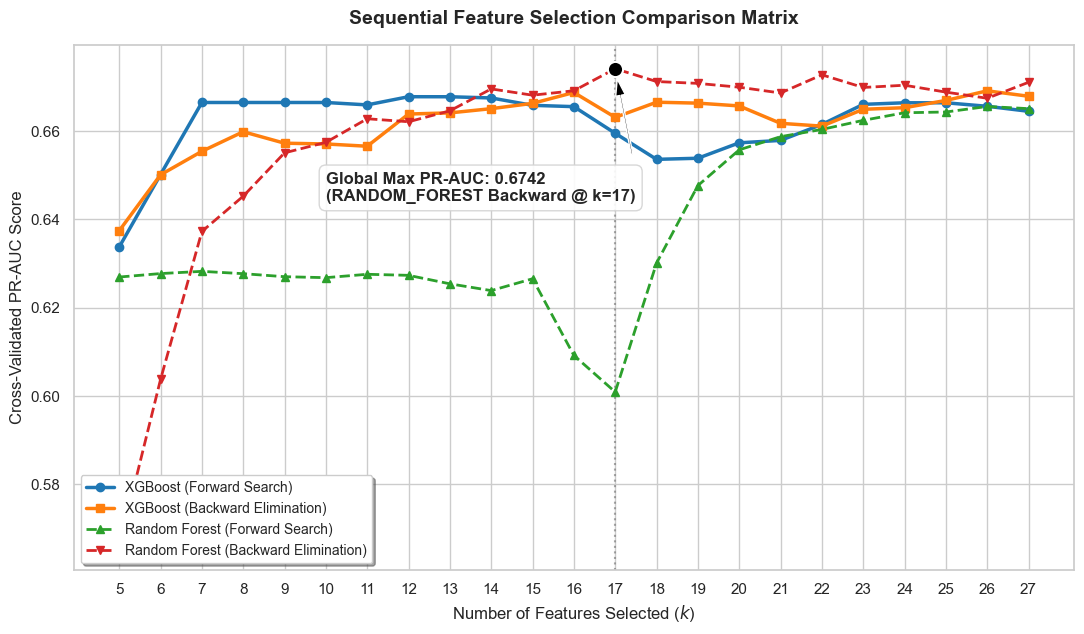
\includegraphics[width=\linewidth]{figures/sequential_feature_selection.png}
\end{columns}
\end{frame}

% ---------------- 17 SELECTED FEATURES ----------------
\begin{frame}{Optimal Feature Subset Analysis}
    \footnotesize
\begin{columns}[T]
\column{0.50\textwidth}
\textbf{Key Domain Findings}
\begin{itemize}\scriptsize
    \item Product density features are retained across all top-performing models.
    \item Cross-product behavioral interactions consistently outperform raw variables.
    \item Financial ratio features catch behavioral drop-offs much more effectively than standalone balance metrics.
\end{itemize}

\column{0.52\textwidth}
\begin{block}{SFS Champion Matrix}
Backward Random Forest selection isolated \textbf{17 core features} to capture the highest baseline predictive resolution (\textbf{0.6742}).
\end{block}
\end{columns}

\centering
\textbf{Feature Group Categories}\\
\footnotesize
\begin{tabular}{ll}
\toprule
\textbf{Category} & \textbf{Extracted Feature Fields} \\
\midrule
Demographics & Gender, Germany, Spain \\
Product Sets & NumOfProducts\_1, 2, 3, 4 \\
Value Metrics & Salary, Point Earned, Satisfaction \\
Interactions & Age$\times$IsActive, CreditScore$\times$Age \\
Ratios & Balance/Product, Credit/Age \\
Card Tiers & Silver Card Type Flag \\
\bottomrule
\end{tabular}

\end{frame}
